\section{Additional diagnostic design and complete summaries}
\label{sec:review2}
The diagnostic protocol is fixed in commit \code{67239e4}, after all first-extension outcomes were known. It defines 120 predictive cells: 80 spline cells (eight settings, two captures, five seeds), ten LR main cells, and 30 forest cells (three conditions, two captures, five seeds). Thirty main cells repeat previous trajectories to check the new runner. They are not additional independent evidence. The first diagnostic attempt was invalidated after a uint8 overflow was found in the guard that determines whether AP is defined. The retained AP diagnostics use the widened integer-count fix and are checked against AUC class-validity coverage, with a dedicated regression test. This affected the new AP diagnostic only; the historical and first-extension reports remain unchanged. The excluded attempt is identified in the provenance log.

\subsection{Operating-point comparisons}
Retrospective interpolation uses observed FPR/recall points within each seed's support. It uses no extrapolation. FPR ties retain the larger recall for a matched-FPR description; recall ties retain the smaller FPR for a matched-recall description. The result is a piecewise-linear description of recorded policies, not an estimated deployment frontier. The CSV includes missing comparisons when a target is outside either controller's observed support. Averaging paired interpolations differs from interpolating seed means because the operating-point locations vary across seeds.
\begin{table}[htbp]\centering\fontsize{8}{10}\selectfont\setlength{\tabcolsep}{3pt}
\caption{Descriptive matched-FPR comparison of the original five cost points on TON D. The paired columns interpolate within each seed, then summarize the supported pairs. Mean-curve columns interpolate curves of seed means. Values are recall percentages; the difference is in percentage points. No comparison extrapolates.}
\begin{tabular}{rrrrrrr}\toprule
FPR & Pairs & Paired frozen & Paired head & Paired difference & Mean-curve frozen & Mean-curve head \\\midrule
\tablerows{tables/review2_matched_rows.tex}\bottomrule\end{tabular}\end{table}
The mean-curve and paired-seed summaries describe different operations. At 13\% FPR, the paired head-minus-frozen difference is $2.41\pm3.11$ percentage points on this stream, whereas the mean curves nearly coincide. These descriptive calculations do not establish equivalence or superiority in a new stream. The low-FPR comparison has incomplete common support. The denser nine-weight audit is retained as additional operating points, without selecting a weight from D for deployment.

With the denser nine-weight grid, the paired head-minus-frozen recall difference at 13\% FPR is $1.49 \pm 3.66$ percentage points (5 supported pairs). This remains a retrospective interpolation within each seed, rather than a threshold selected for a new stream.


\subsection{Model audit and threshold transfer}
Model audits verify that label one denotes an attack and higher scores denote greater attack confidence. LR coefficients, decision-function output, and the attack-probability column are checked directly. Cached D scores are checked on 5,000 fixed sampled observations against direct model predictions. Full A/B/D fixed-score metrics and class-specific score quantiles are retained. A metrics describe the training population, not generalization. Chronological ARF initial fitting and its shuffled control use exactly the same sampled row set; only their order changes.

The fixed LR class ordering is $[0,1]$. Coefficient scores and the attack-probability column agree numerically with the cached score; the full audit records the maximum discrepancies and solver iteration counts. On TON the inversion is already visible on B, before D. This supports poor temporal transfer within the compact feature contract, rather than an implementation that systematically reverses the attack label.

For frozen spline thresholds, the following summaries weight each calibration/next-block pair by the next block's normal count and exclude the initial period before valid calibration. TON, $\lambda=1$: calibration FPR 42.67\%, next-block FPR 48.30\%; median distinct normal scores 55. TON, $\lambda=2$: calibration FPR 8.26\%, next-block FPR 13.20\%; median distinct normal scores 55. UNSW, $\lambda=1$: calibration FPR 2.67\%, next-block FPR 5.64\%; median distinct normal scores 110. UNSW, $\lambda=2$: calibration FPR 2.36\%, next-block FPR 5.16\%; median distinct normal scores 110. The calibration and future populations differ; these are descriptive transfer diagnostics, not estimates of independent calibration-sample uncertainty. Distinct scores can be much fewer than retained normal observations.


\subsection{Conditional ranking and precision--recall summaries}
AP is noninterpolated average precision. AP is recorded for the main, shuffled, and FIT-only conditions; the seven spline sensitivity conditions retain AUC and confusion counts. Blocks containing only one class are excluded from within-block AUC/AP summaries; their counts and class coverage are explicit in the CSV. Macro AP is not pooled AP, and weighting block AP by class counts does not turn it into pooled AP. Precision at each operating policy is computed from globally summed confusion counts. Comparisons across captures must account for their different prevalence.
\begin{table}[htbp]\centering\fontsize{7.5}{9.5}\selectfont\setlength{\tabcolsep}{3pt}
\caption{Ranking summaries, mean $\pm$ seed SD conditional on each capture. NW and AW denote normal-count and attack-count weighting of valid blocks. Adaptive rows use the chronological initialization and default controller.}
\begin{tabular}{lllrrrrr}\toprule
Stream & Model & Score & AUC macro & AUC NW & AP macro & AP NW & AP AW \\\midrule
\tablerows{tables/review2_ranking_rows.tex}
\bottomrule\end{tabular}\end{table}

\subsection{Forest feedback and persistent state}
\begin{table}[htbp]\centering\small\setlength{\tabcolsep}{4pt}
\caption{Forest label and state ledger, mean $\pm$ SD conditional on each capture. Learned labels count D arrivals used once for learning, excluding initial A fitting. Final serialized model size excludes external controller memory and is not peak RAM.}
\begin{tabular}{llrrr}\toprule Stream & Condition & Acquired labels & Learned labels & Final model MiB \\\midrule
\tablerows{tables/review2_forest_ledger_rows.tex}\bottomrule\end{tabular}\end{table}
Standard and shuffled forests reuse CAL-role labels for learning. The FIT-only condition excludes those labels throughout D, while retaining the same chronological initial state. The acquired budget remains shared even though fewer labels enter learning. Per-seed timings are retained in the CSV; runs execute concurrently, so those timings are audit records rather than a controlled hardware benchmark.

\subsection{Memory, age, eligibility, and role-salt sensitivity}
One factor changes at a time. The default is FIT192/CAL64, age 50, minimum five CAL observations per class, and salt \code{ADAPT04-C-seed42-v1}. Labels continue to arrive after prediction, and all configurations use the same query sequence for each dataset/seed. The age factor also applies to the independent all-label CAL256 control. FIT entries have no age filter. Capacity variants preserve the nominal 3:1 FIT/CAL allocation but change the total retained examples to 128 or 512. Alternative salts are literal \code{review2-salt-1} and \code{review2-salt-2}; the same alternative is used for all five seeds. No setting is chosen as a new primary configuration from D results.
\begin{table}[htbp]\centering\small\setlength{\tabcolsep}{4pt}
\caption{Spline head/CAL sensitivity. Rates are percentages, mean $\pm$ sample SD conditional on each stream. Updates are mean valid transactions. Main denotes the default.}
\begin{tabular}{llrrrr}\toprule
Stream & Changed setting & Recall & FPR & BA & Updates \\\midrule
\tablerows{tables/review2_sensitivity_rows.tex}
\bottomrule\end{tabular}\end{table}

\subsection{Complete first-extension default comparisons}
The following tables retain all displayed default model comparisons from the first extension. Each seed describes the same captured stream. Frozen LR and chronological ARF quality must be interpreted using the audits in the main paper; the macro AUROC column is accompanied by normal-weighted and pooled summaries elsewhere in this Supplement.
\begin{table}[htbp]\centering\fontsize{8.8}{10.5}\selectfont\setlength{\tabcolsep}{4pt}
\caption{TON first-extension defaults. Rates are percentages, mean $\pm$ SD conditional on one stream; AUROC is the macro mean over valid prediction blocks.}
\begin{tabular}{lrrrr}\toprule Controller & Recall & FPR & BA & AUROC \\\midrule
\tablerows{tables/ton_extension_rows.tex}\bottomrule\end{tabular}\end{table}
\begin{table}[htbp]\centering\fontsize{8.8}{10.5}\selectfont\setlength{\tabcolsep}{4pt}
\caption{UNSW first-extension defaults, with the same conditional reporting convention.}
\begin{tabular}{lrrrr}\toprule Controller & Recall & FPR & BA & AUROC \\\midrule
\tablerows{tables/unsw_extension_rows.tex}\bottomrule\end{tabular}\end{table}
\begin{figure}[htbp]\centering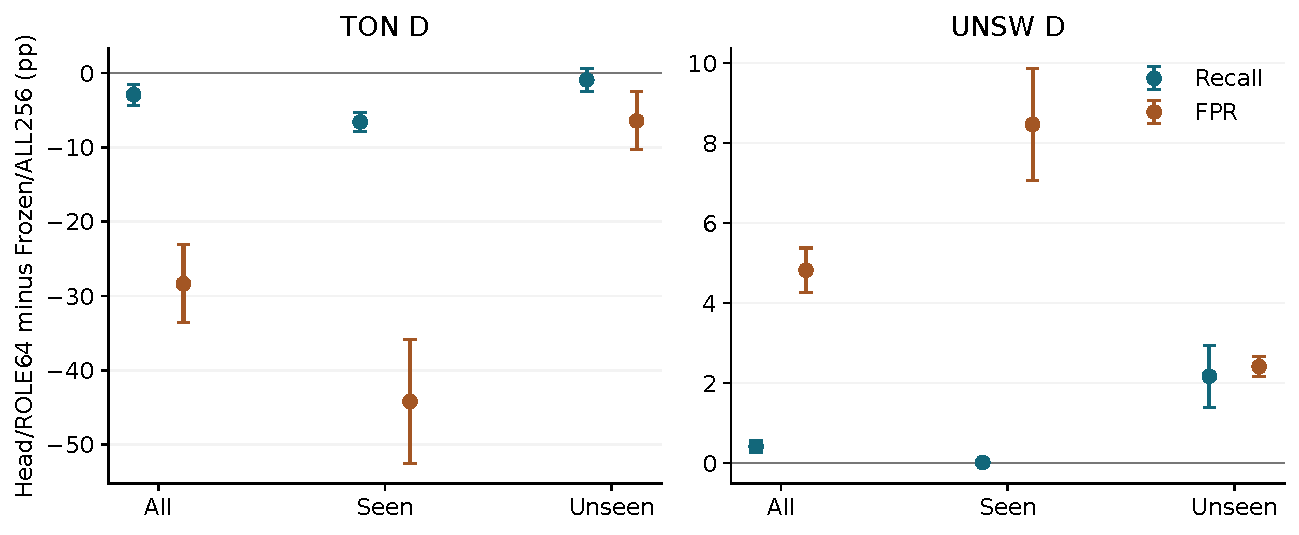
\includegraphics[width=\linewidth]{figures/fig6_stratum_effects.pdf}
\caption{Spline head/CAL64 minus Frozen/CAL256 at $\lambda=1$ in the first extension, by representation-recurrence stratum. Points are paired seed means and bars are sample SD on the same stream. Positive recall and negative FPR changes favor the head; concurrent reductions describe fewer false alarms at the expense of recall.}
\end{figure}
\FloatBarrier
\subsection{Additional first-extension controls}
\begin{table}[htbp]\centering\small\setlength{\tabcolsep}{4pt}
\caption{Independent CAL64, offset-only and prior-centred spline controls. Mean $\pm$ SD describes five randomizations on one stream.}
\begin{tabular}{llrrr}\toprule Dataset & Controller & Recall & FPR & BA \\\midrule
\tablerows{tables/ablation_rows.tex}\bottomrule\end{tabular}\end{table}
Independent CAL64 produces the same outcomes as the matched CAL64 schedule in these main runs. Offset/CAL64 produces the same decisions as frozen/CAL64, as expected from $s+c>\tau+c$ being equivalent to $s>\tau$. The prior-centred refit minimizes summed logistic loss plus $\tfrac12\lVert w-w_{\rm previous}\rVert^2$, with an unpenalized intercept. Its BA is 84.42\% on TON and 93.72\% on UNSW, compared with 84.84\% and 93.22\% for the default head. It supplies no uniform remedy across the two captures.
\begin{table}[htbp]\centering\fontsize{8.5}{10}\selectfont\setlength{\tabcolsep}{3.4pt}
\caption{First-extension TON delay and budget sensitivity, conditional on the same stream. Default budget is 1\%; only the final pair uses 0.1\%. Updates include the final transaction without a subsequent evaluated block.}
\begin{tabular}{llrrrr}\toprule Condition & Controller & Recall & FPR & BA & Updates \\\midrule
\tablerows{tables/sensitivity_rows.tex}\bottomrule\end{tabular}\end{table}
\FloatBarrier
